\subsubsection{\gls{AS}}
\textbf{Ansvar}\\
\gls{AS} er den del af systemet, hvor produktkataloget bliver redigeret. Dette indebærer oprettelse, sletning og ændring af produkter, såvel som produktkategorier. \gls{AS} bliver betjent af \gls{SB}, se aktørkontekst diagram, figur \ref{fig:aktcont} side \pageref{fig:aktcont}.\\

\textbf{Sekvensdiagram}
\begin{figure}[H]
	\centering
	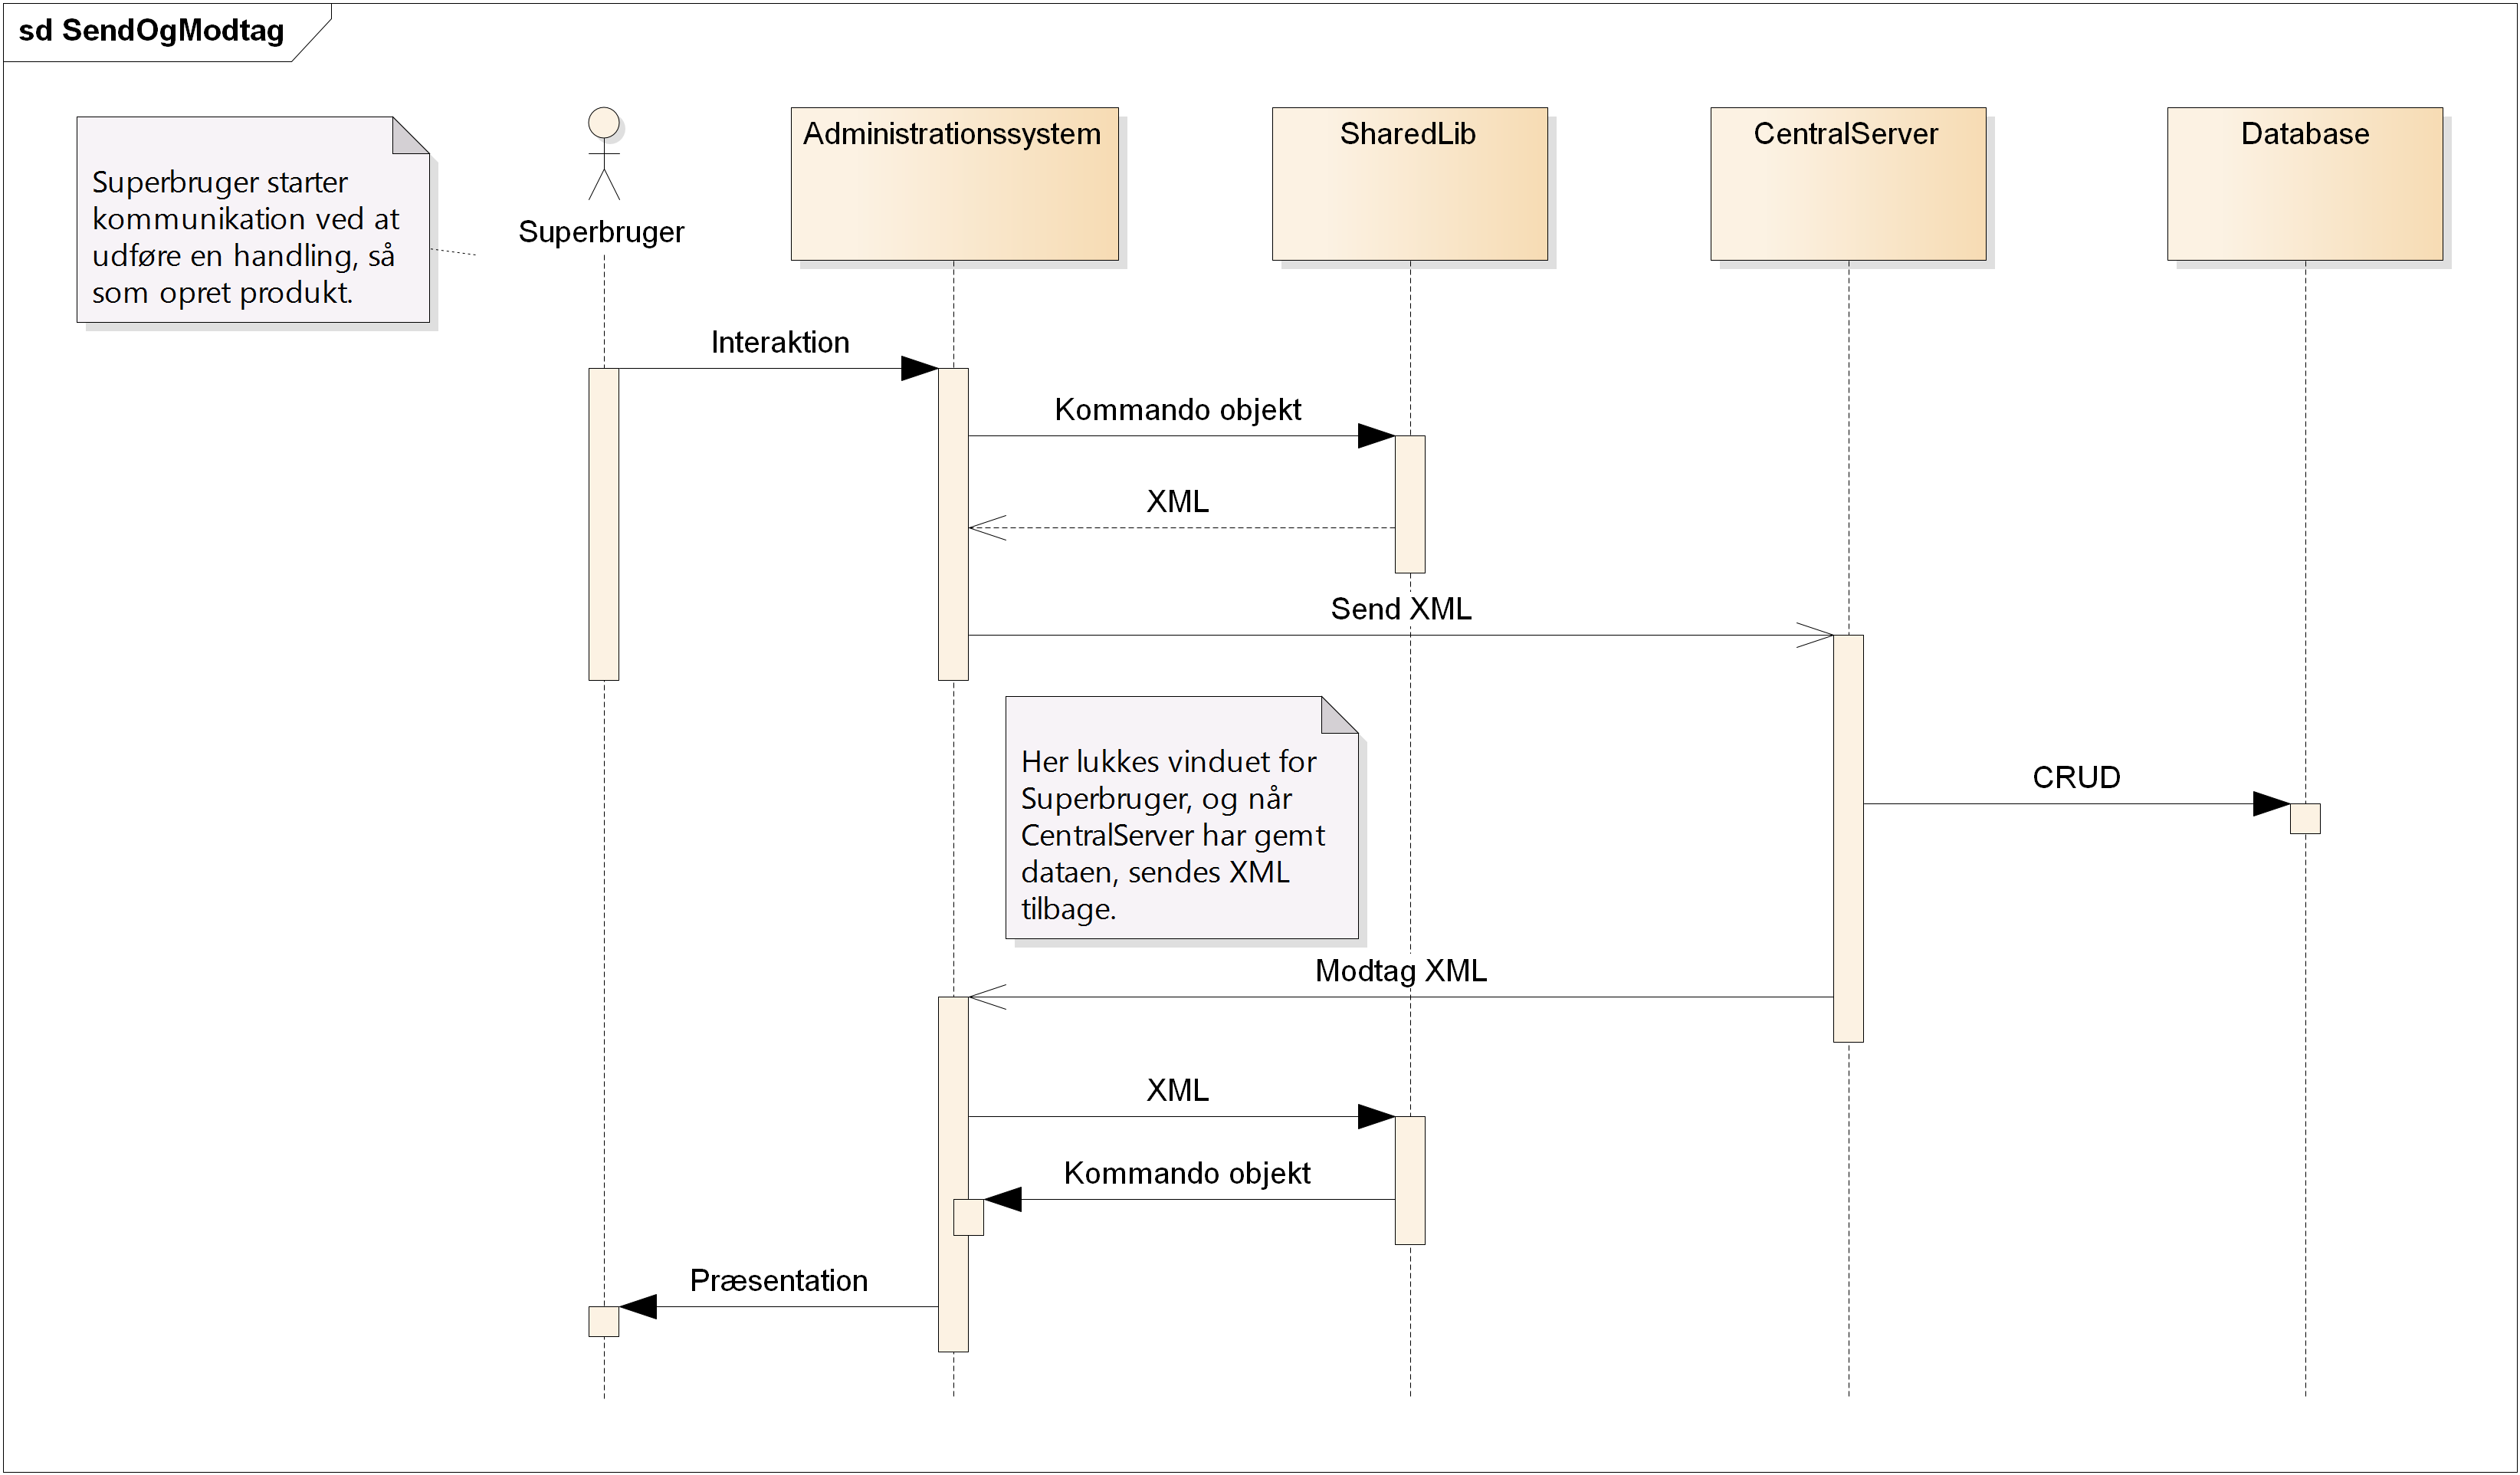
\includegraphics[width=\textwidth]{Systemarkitektur/LogiskView/Administrationssystem-sekvensdiagram}
	\caption{Sekvensdiagram for kommunikation mellem \gls{AS} og andre pakker}
	\label{fig:logview_admin_sekvensdiagram}
\end{figure}

Sekvensdiagrammet på figur \ref{fig:logview_admin_sekvensdiagram} viser den kommunikation der foregår mellem \gls{AS}et og de andre pakker i systemet. \gls{AS}et kommunikerer udelukkende med \gls{CS}, mens \gls{SL} bliver brugt til at encode og decode XML strenge der sendes og modtages fra \gls{CS}. Sekvensdiagrammet (figur \ref{fig:logview_admin_sekvensdiagram}) viser udelukkende interfacet mellem pakkerne. Uddybende forklaring af \gls{AS} pakken kan findes under dens designafsnit, se afsnit \ref{section:design_admin}.

